\hypertarget{tyuxf6n-teoriataustaa}{%
\chapter{Työn teoriataustaa}\label{tyuxf6n-teoriataustaa}}

\hypertarget{section}{%
\section{\texorpdfstring{\Gls{ddd}}{}}\label{section}}

Yleinen ongelma tietokoneohjelmistoja tehtäessä on, että ohjelmoijat
tuntevat ohjelmiston erikoisalan heikosti. Esimerkiksi
kiinteistötekniikkaa, kirjastokortistoa tai tämän työn tapauksessa
terapiaklinikan toimintaa hoitavan ohjelmiston kehittäjä joutuu
käsittelemään monimutkaisia, sovellusalaan sidottuja ongelmia. Näiden
alojen asiantuntijat puolestaan tietävät, miten sovellusalan ongelmat
ratkaistaan, mutta heiltä puuttuu taito suunnitella ohjelmistoja.

Tämän ongelman ylittäminen on aihe, jota Eric Evans käsittelee
kirjassaan Domain Driven Design\cite{evans:ddd}. Evansin mielestä
jokaisen monimutkaisemman ohjelmiston sisässä on \gls{domainmodel}
(Domain model), eli malli siitä, miten kyseinen ohjelmisto ratkaisee
sovellusalan ongelmat. Malli voi kuitenkin olla piilossa ohjelmakoodin
sisällä, ja saattaa olla, etteivät ohjelmiston kehittäjät edes tiedosta
mallin olemassaoloa. Tämän mallin tuominen näkyväksi on
sovellusaluevetoisen suunnittelun päätavoite.

\Gls{crunching} (Knowledge crunching) on keskeinen väline
sovellusaluemallin rakentamiseen. Evans kuvaa prosessin, jossa
kehittäjät luonnostelevat yhdessä sovellusalueen asiantuntijoiden kanssa
\glsdisp{domainmodel}{sovellusaluemallin}. Tämä prosessi on
tyypillisesti kehittäjien vetämä, ja se koostaa yhteen informaatiota
monenlaisista lähteistä: sovellusalueen asiantuntijoilta, järjestelmän
käyttäjiltä, ohjelmoijien aiemmasta kokemuksesta jne.

Malli kytketään tiiviisti yhteen ohjelmakoodin kanssa vuorottelemalla
suunnittelun ja ohjelmistokehityksen välillä. Varhaiset
prototyyppiversiot ohjelmistosta toimivat jatkosuunnittelun
materiaalina. Kun prosessia jatketaan, malli muuttuu ja syvenee. Evansin
mukaan tämä on seurausta siitä, että ohjelmoijien ymmärrys
sovellusalueesta syvenee.\cite{evans:ddd}

Tavoitteena on, että ohjelmistokehittäjien ja alan asiantuntijoiden
välille rakentuu \gls{ubilang}, jonka avulla kaikkien on mahdollista
yhteisesti keskustella ohjelmiston toiminnasta ja kehitystarpeista.
\gls{ubilang} yhdistää ja yhdenmukaistaa myös ohjelmiston eri osien
parissa toimivien kehittäjien kielenkäyttöä.

Kaikenkattavan kielen käsitteitä ovat luokkien nimet ja ohjelmiston
keskeiset operaatiot. Se myös sisältää käsitteet, joilla voidaan kuvata
käsitteiden käyttöä rajoittavat ja hallinnoivat keskeiset säännöt.
Kaikenkattavan kielen käsitteet elävät ohjelmakoodissa, ja muodostavat
koodin ytimessä sijaitsevan \glsentryname{domainmodel}in.

Evans painottaa, että kaikenkattavaan kieleen tehtävä muutos muuttaa
myös \glsentryname{domainmodel}ia ja ohjelmakoodia.

Koodina kuvattu \glsentryname{domainmodel} tulee myös eriyttää
ohjelmassa omaksi arkkitehtuuriseksi tasokseen. Onnistuneesti erotettu
sovellusalakohtainen logiikka muodostaa sovelluksen
\glslink{domainlayer}{liiketoimintalogiikan tason} (Domain layer).

\hypertarget{rakennuspalikat}{%
\subsection{\texorpdfstring{\glsdisp{ddd}{Sovellusaluevetoisen suunnittelun}
rakennuspalikat}{ rakennuspalikat}}\label{rakennuspalikat}}

Koska Evansin lähtökohta on, että \glsentryname{domainmodel} ilmaistaan
nimenomaan ohjelmakoodin kautta, tarvitaan joukko käytännön työkaluja,
joiden avulla \glsentryname{domainmodel} on mahdollista toteuttaa
teknisesti. Käyn seuraavaksi läpi muutamia keskeisimpiä.

\Gls{entity} edustaa käytännössä kaikkea, jolla on identiteetti.
Esimerkiksi kahdella ihmisellä voi olla sama nimi, mutta he ovat silti
identiteetiltään eri henkilöitä. \glsentryname{entity} voi myös muuttaa
muotoaan, esimerkiksi ihminen kasvaa aikuiseksi ja vaikkapa vaihtaa
sukunimensä. Identiteetti säilyy silti. Todella suuri osa
\glsentryname{domainmodel}{sta} koostuu juuri
\glsdisp{entity}{yksilötyypeistä}, sillä niitä on suurin osa
kaikenkattavan kielen käsitteistä.

Esimerkiksi terapeutin kahdesta eri hoitokäynnistä luomilla laskuilla on
identiteetti. Kahdella laskulla voi olla sisällytettynä samat
hoitotoimenpiteet ja maksajakin voi olla sama, mutta silti laskut ovat
omia erillisiä kokonaisuuksiaan.

Käsitteiden lisäksi tärkeä osa mallia ovat käsitteiden väliset suhteet.
Tosielämässä kaikki liittyy kaikkeen, mutta sovellusalueen sisäinen
logiikka tarvitsee vain osajoukon kaikista suhteista toimiakseen.
Huolellisesti valitut suhteet käsitteiden välillä paljastavat
hyödyllistä tietoa mallin perimmäisestä tarkoituksesta.

Myös \gls{kulkusuunta} \glsdisp{entity}{yksilötyyppien} välillä on
tärkeä. Se vaikuttaa paitsi ohjelmiston tekniseen monimutkaisuuteen,
myös siihen, minkälaisia asioita mallilla on mahdollista ilmaista.

Esimerkiksi käynnin ja laskun välinen suhde voi olla yksi- tai
kaksisuuntainen, ja tämä vaikuttaa huomattavasti ohjelmiston toimintaan.

\begin{itemize}
\tightlist
\item
  Tapaus A: käynniltä löytyy tieto, mille laskulle se on lisätty, mutta
  lasku ei osaa kertoa, mikä käynti sillä on laskutettuna.
\item
  Tapaus B: lasku tietää, mikä käynti sille on lisätty, mutta käynniltä
  ei voi kysyä, millä laskulla se on.
\end{itemize}

Kolmas vaihtoehto on mahdollistaa kulkeminen molempiin suuntiin näiden
kahden käsitteen välillä. Tällöin malli on monipuolisempi, mutta myös
ohjelman tekninen monimutkaisuus kasvaa. Mikäli käsitteiden väliset
suhteet on toteutettu teknisesti viittauksina olioiden välillä,
viittauksia täytyy päivittää mahdollisesti kahteen eri paikkaan, ja
lisäksi varoa, ettei viittauksista muodostu kehämäisiä. Onkin tärkeää
pyrkiä rajoittamaan olioiden väliset suhteet ja kulkusuunnat
mahdollisimman vähäisiksi, jotta ohjelma pysyy teknisesti mahdollisimman
yksinkertaisena.

Toisinaan sovellusalueeseen kuuluvat oliot muodostavat ryhmiä, joissa
yksi olio on juuriolio, ja muut riippuvat tästä. Tällaisia ryhmiä Evans
kutsuu nimellä \gls{aggregate}. Esimerkiksi laskurivi on hyödytön ilman
laskua, jolle se kuuluu. Lasku ja laskurivi muodostavatkin aggregaatin -
kokonaisuuden, jota käsitellään aina ryhmänä. Esimerkiksi tietokannasta
ei kysytä yksittäisiä laskurivejä, vaan aina ensiksi lasku, ja sitten
siihen kuuluvat rivit. Samoin ohjelmassa ei anneta suoraa viittausta
laskuriviin laskun ulkpuolelle, vaan laskurivin kanssa toimiminen
tapahtuu laskun tarjoamien toimintojen kautta.

Kun monimutkaisempia sovellusalueen käsitteitä koostetaan, on toisinaan
hyödyllistä siirtää koostamistyö kokonaan erilliseksi oliokseen. Näitä
olioita Evans kutsuu tehdas-luokiksi (factory), samaan tapaan kuin
olio-ohjelmoinnin perinteessä muutenkin. Tehdas-luokan tehtävänä on
koostaa useasta alikäsitteestä koostuva kokonaisuus.

Esimerkiksi laskulla voi olla maksaja, joukko laskutettavia asioita, ja
niitä vastaavat laskurivit ja juokseva numerointi. Tällaisen
kokonaisuuden rakentaminen ei enää onnistu yksinkertaisella laskun
luontikomennolla, vaan tarvitaan erillinen tehdas-luokka, jolta voi
pyytää eri tavoin rakennettuja laskuja. Tämä luokka voi varmistaa, että
jokainen lasku saa uniikin numeronsa, että kaikki laskuun kuuluvat
laskurivit ovat paikallaan ja että maksajan perustiedot ovat myös
laskulla mukana ja käytettävissä.

Mielenkiintoinen käsite Evansilla on \gls{repository}. Se edustaa
projektissa tiedon tallennuspaikkaa, kuten vaikka tietokantaa. Ajatus
on, että \glsdisp{domainmodel}{sovellusaluemallin} tasolla ei esitetä
konkreettista tiedontallennustoteutusta, vaan ainoastaan abstrakti
tietovarasto , \emph{repositorio}. Tähän repositorioon on mahdollista
kohdistaa erilaisia hakuja sekä muokkausoperaatioita, ja repositorio
palauttaa käytettäväksi kokoelman olioita, jotka edustavat
\glsdisp{domainmodel}{sovellusaluemallin} käsitteitä.

Esimerkiksi laskut on mahdollista hakea laskurepositoriosta, johon on
toteutettu tarvittavat hakumetodit esimerkiksi laskunumeron tai laskun
päiväyksen perusteella. Näin sovellusaluemallia kehitettäessä ei
tarvitse pohtia, mihin tieto on tallennettu ja millaisella kyselyllä se
haetaan. Esitän listauksessa \ref{repository} hyvin yksinkertaisen
repositorioluokan laskujen hakemiseksi.

\begin{code}
  \begin{minted}{python}
  
  Class InvoiceRepository:
  
    def get_all():
      return self.invoices
      
    def find_by_date(date)
      return self.invoices.filter(date)

\end{minted}
\captionof{listing}{Yksinkertainen esimerkki abstraktista repositoriosta.}
  \label{repository}
\end{code}

Esitetty repositorio tallentaa tiedon vain olion sisään, mutta metodit
voisivat yhtä hyvin sisältää esimerkiksi SQL-kutsuja, tai jonkin
ORM-järjestelmän käyttökutsuja.

\hypertarget{mallin-hiominen-refaktoroimalla}{%
\subsection{Mallin hiominen
refaktoroimalla}\label{mallin-hiominen-refaktoroimalla}}

Refaktoroinnilla tarkoitetaan koodin rakenteen muuttamista niin, että
koodin tuottama tulos ei muutu. Refaktoroimalla voi siistiä koodia ja
tehdä siitä luettavampaa.

Evansin mukaan hyvä \glsentryname{domainmodel} syntyy hyvin harvoin
ilman refaktorointia. Hän ei tarkoita refaktoroinnilla pelkästään koodin
teknistä siistimistä, vaan refaktoroinnin motivaationa on tuoda
\glsentryname{domainmodel} paremmin näkyviin koodin tasolla. Tämä vaatii
joustavasti kirjoitettua koodia, jota on helppo
muunnella.\cite[osa 3.]{evans:ddd}

Keskeinen keino joustavan koodin tuottamiseksi ovat edeltäkäsin
kirjoitettavat yksikkötestit. Kun testi laaditaan ennen koodin
kirjoittamista, koodin keskinäiset kytkökset muodostuvat löyhiksi.
Testien suoritustiheys on myös oleellista. Parhaisiin tuloksiin päästään
jatkuvalla testaamisella. Se on menetelmä, jossa testityökalu tarkkailee
lähdekooditiedostojen muutoksia, ja suorittaa testipatteriston uudelleen
joka kerta, kun koodiin tulee muutoksia. \cite[luku 6]{beck2004extreme}

Kattavasti yksikkötestattua koodia on myös helppo muunnella. Sen
rakenteeseen ja toimintaan voi tehdä suuriakin muutoksia, ilman että
tarvitsee pelätä takaiskuja. Tämä edellyttää, että testit ovat siistejä
ja vähäeleisiä, ja kirjoitettu samalla tarkkuudella kuin tuotantokoodi.
Paras metodi tähän tulokseen pääsemiseksi on kirjoittaa testejä ja
tuotantokoodia rinnakkain rivi riviltä. Ohjenuorana voi käyttää ns.
testipohjaisen kehittämisen kolmea sääntöä. Ne ovat: 1. Tuotantokoodia
ei saa kirjoittaa, ennenkuin on kirjoittanut epäonnistuvan yksikkötestin
2. Yksikkötestiä saa kirjoittaa vain sen verran kuin vaaditaan sen
epäonnistumiseen. Kääntäjän tai tulkin raportoima virhe lasketaan
epäonnistumiseksi. 3. Tuotantokoodia saa kirjoittaa vain sen verran,
että yksikkötesti menee läpi.\cite[luku 9]{martin2008clean}

Joustavan järjestelmän suunnittelussa on myös hyvä seurata nk.
YAGNI-periaatetta\footnote{``You Aren't Gonna Need It.'' suom. ``Et sinä
  sitä tarvitse.''}. Kyseinen periaate edellyttää, että vain sellainen
koodi kirjoitetaan, jolle on tarvetta. Luokkiin tai moduuleihin ei
lisätä metodeita eikä toimintoja varmuuden varalta. \cite{jeffries1998}

Evans toteaa, että joustava rakenne on monesti seurausta siitä, että
\gls{domainmodel} kehittyy paremmaksi. Joustava ohjelmisto ei ole
monimutkainen, eikä se piilota toiminnallisuuksiaan outojen rajapintojen
taakse. Joustava ohjelmisto koostuu mahdollisimman pienestä määrästä
löyhästi toisiinsa kytkeytyviä käsitteitä.\cite[luku 10]{evans:ddd}

\hypertarget{graphql-teknologian-kuvaus}{%
\section{GraphQL-teknologian kuvaus}\label{graphql-teknologian-kuvaus}}

Useimmat sovellukset ovat nykyään web-sovelluksia, ja useimmat
web-sovellukset puolestaan perustuvat \glsentryname{rest}
(Representational State Transfer) -rajapintoihin. \glsentryname{rest} on
arkkitehtuurityyli, jossa palvelin esittää asiakasohjelmalle joukon
resursseja, joita asiakasohjelma voi pyytää ja muunnella tilattomia
pyyntöjä käyttäen.\cite{fielding2000architectural}

REST-tyyli on vakiintunut web-sovellusten toteuttamisteknologiaksi,
mutta siihen liittyy myös eräitä ongelmia. Mikäli REST-tyyppisestä
rajapinnasta halutaan hakea usean eri resurssin verkko, joudutaan
tekemään erillinen pyyntö jokaista resurssia kohti. Toisissa tapauksissa
taas halutaan vain osa resurssin esittämästä tiedosta, mutta joudutaan
silti hakemaan koko
resurssi.\cite{betterRESTPrisma}\cite{WhyUseGraphQLApollo}

\gls{graphql} on Facebookin kehittämä kyselykieli, jolla
edellämainittuja ongelmia pyritään ratkaisemaan. Sen alkuperäinen
suunnitteluperiaate oli tarjota web-asiakasohjelmien kehittäjille
aiempaa laajempi vapaus rajapintapyyntöjen laatimiseen. GraphQL esittää
datan olioiden keskinäisenä verkkona. \cite{graphql:spec}

GraphQL on vielä suhteellisen uusi teknologia, eikä siitä löydy kovin
paljoa materiaalia. Keskeinen tiedonlähde ovat
Facebookin\cite{graphql:spec} ja GraphQL-säätiön\cite{GraphQLOrg}
julkaisemat verkkomateriaalit, sekä Apollo Graph -yrityksen
GraphQL-teknologiaa käsittelevä materiaali.\cite{ApolloGraphQL}

GraphQL koostuu kahdesta osasta: kyselykielestä sekä
tyyppijärjestelmästä. Kyselykielellä muotoillaan pyyntö, johon
GraphQL-palvelun tulee vastata. Tyyppijärjestelmä taas tarkistaa pyynnön
oikeellisuuden.

GraphQL ei ole varsinainen rajapinta, sillä palvelun
toteuttamisteknologia on määrittelyn ulkopuolella. Useimmiten
GraphQL-palvelut on toteutettu \gls{http}-teknologian päälle, mutta
muitakin, kuten WebSocketia, voi käytttää. GraphQL ei myöskään
määrittele, miten kyselyn vastaus tulee muodostaa, tai milllä
ohjelmointikielellä järjestelmä tulee toteuttaa.

Aivan täysin kielineutraali GraphQL ei silti ole. Osa konventioista on
JavaScript-konventioita. Esimerkiksi kentän- ja muuttujien nimet on
tapana kirjoittaa camelCase- ja PascalCase -muodoissa, eli vaihdellen
suuria ja pieniä kirjaimia sanan sisällä samoin kuin kyseiset sanat
tässä virkkeessä on tehty.\cite{GraphQLSchemaBasics}

\hypertarget{verkoista}{%
\subsection{Verkoista}\label{verkoista}}

GraphQL esittää datan olioiden välisenä verkkona.

\gls{verkko} eli graafi on tietorakenne, joka koostuu N:stä solmusta ja
niitä yhdistävistä kaarista.\cite{pozrikidis2014introduction} Verkkojen
avulla on mahdollista esittää monenlaisia asioiden välisiä suhteita,
kuten esimerkiksi reittikartta usean kaupungin välisistä teistä.

Olio-ohjelmoinnin tyyli esittää ratkaistavan ongelmakentän olioiden
välisinä verkkoina. Ohjelmassa ei ole juuri lainkaan jaettua tilan
käsittelyä, vaan kaikki tai lähes kaikki ohjelman sisältämä tieto on
olioissa. Näin käsiteltävät ongelmakokonaisuudet saadaan jaettua
pienempiin, hallittavan kokoisiin osiin. \cite{booch2008object}

GraphQL:n avulla sovellusala on mahdollista esittää verkon muodossa
määrittelemällä GraphQL-tyyppien verkko. Tämän avulla rajapinta tarjoaa
asiakasohjelmalle rakenteen, joka muistuttaa olio-ohjelmoinnin
olioverkkoja.\cite{thinkingInGraphs}

Juuri verkkorakenne tekee olio-ohjelmoinnista tehokkaan välineen
tosielämän ongelmien ratkaisemiseen. Oliot voivat edustaa ohjelman
\gls{domainmodel}n käsitteitä, ja verkko muodostaa niiden välisen
käsitekartan.

Käsitteiden verkkoa kuvaa myös Eric Evans Domain Driven Design
-kirjassa. Keino rakentaa \glsentryname{ubilang} kehittäjien ja alan
asiantuntijoiden välille on antaa tärkeille käsitteille nimet, sijoittaa
ne mallissa oikeisiin suhteisiin keskenään ja myös toteuttaa ne
koodissa.

Jotta tietokone saa käsitteistä täyden hyödyn irti, on käsitteet
jaettava muodollisesti määritettyihin tyyppeihin.

\hypertarget{tyyppijuxe4rjestelmuxe4}{%
\subsection{Tyyppijärjestelmä}\label{tyyppijuxe4rjestelmuxe4}}

Tietokoneet käsittelevät dataa ottamatta sen enempää kantaa sen
\glsdisp{tyyppi}{tyyppiin}. Pohjimmiltaan data on vain bittijonoja
muistissa, tai elementtejä joukossa. Kun tällaista järjestämätöntä ja
tyypittämätöntä joukkoa ryhdytään käsittelemään, on välttämätöntä
järjestää se erilaisiin kategorioihin. Tämä tiedon luokittelu synnyttää
tyyppijärjestelmän, mutta järjestelmä ei ole formaalisti määritelty,
eikä tietokone voi niin ollen tehdä tyyppitarkistusta.

Tyypitys tarkoittaa määrättyjä rajoituksia, joiden avulla voidaan
varmistaa muuttujan oikeellisuus. Staattinen tyypitys on menetelmä,
jossa lausekkeiden tyyppi voidaan määrittää staattisen analyysin avulla,
siis jo käännösaikaisesti. Vahva tyypitys taas mahdollistaa tyypin
tarkistamisen luotettavasti ajon aikana. \cite{Cardelli+Wegner:1985}

GraphQL-rajapinta koostuu tyypeistä, joita rajapinnalle lähetettävä
kysely käyttää. Kyselyssä määritetään pyydettävät tyypit ja niiden
kentät. Rajapinta palauttaa takaisin oliota edustavan joukon kenttiä
\gls{hakurakenne}-muodossa, eli tietorakenteena, joka koostuu avain-arvo
-pareista. \cite{graphql:spec}

GraphQL:ää käyttävät sovellukset on kuitenkin useimmiten kirjoitettu
dynaamisesti tyypitetyillä kielillä, jotka eivät sisällä
tyyppitarkistuksia, tai tarkistukset ovat ajonaikaisia ja vapaaehtoisia.
Esimerkiksi alkuperäinen GraphQL-referenssi-implementaatio on
kirjoitettu JavaScriptillä.\cite{graphqlRefImple2021Oct}

Samoin Python-kieli on dynaamisesti tyypitetty, ja olioiden
tunnistamisessa se käyttää duck-tyypitykseksi kutsuttua menetelmää.
Duck-tyypityksessä olion tyyppiä ei tarkasteta välttämättä edes
ajonaikaisesti, vaan oletetaan sen sisältämien jäsenten
perusteella.\cite{pythonGloss2021Oct} Jos esimerkiksi oliosta löytyvät
kentät \emph{summa} ja \emph{laskunumero}, oletetaan, että olio on
lasku.

Tässä mielessä voidaan ajatella, että GraphQL on keino tuoda
ajonaikaisia tyyppitarkistuksia myös dynaamisesti tyypitetyillä kielillä
kirjoitettuun sovellukseen. Rajapinta erottaa toisistaan ohjelmiston
taustaosan ja käyttöliittymän, joten tällä rajalla tehtävän
tyyppitarkistuksen voi ajatella ehkäisevän virheitä ja parantavan
ohjelmiston luotettavuutta.

Oheisessa koodiesimerkissä \ref{listing1} kuvaan rajapinnan edustamien
tyyppien, ja sitä myötä sen palauttamien olioiden väliset suhteet.
ConsolidatedInvoice-tyyppisessä oliossa on sisällä invoices-kenttä, joka
on lista Invoice-tyyppisiä olioita.

Laskutuksessa ConsolidatedInvoicella eli koontilaskulla tarkoitetaan
yhdistelmälaskua, joka kokoaa yksittäisiä laskuja (Invoice).

Tältä rajapinnalta voi pyytää listaa koontilaskuista. GraphQL:n
tyyppijärjestelmä takaa, että koontilaskun sisällä on invoices-jäsen,
joka sisältää listan Invoice-tyyppisiä olioita, eli siis laskuja.

\begin{code}
  \begin{minted}{graphql}

type Query {
  consolidatedInvoices [ConsolidatedInvoice]
}

Type Invoice {
  number: Int
  sum: Float
  date: Date
}

type ConsolidatedInvoice {
  number: Int
  invoices: [Invoice]
}
  \end{minted}
\captionof{listing}{Esimerkki GraphQL-skeemasta, joka määrittelee yksinkertaisen rajapinnan.}
  \label{listing1}
\end{code}

\hypertarget{skeema}{%
\subsection{Skeema}\label{skeema}}

GraphQL:n olioverkko kuvataan täsmäkielellä määritellyn skeeman avulla.

\Gls{dsl} on ohjelmointikieltä korkeamman tason kieli, joka on
suunniteltu jollekin kapealle sovellusalueelle.\cite{landin1966next}
Esimerkkejä \glsentryname{dsl}istä ovat esimerkiksi UNIX-tyyppisistä
järjestelmistä tutut \emph{sed}- ja \emph{awk}-kielet. Tällaisen kielen
avulla on mahdollista määritellä monimutkaisiakin asioita
nopeasti.\cite{Raymond2003} Kieli tarjoaa tavanomaista ohjelmointikieltä
ilmaisuvoimaisemman ja täsmällisemmän tavan määritellä asioita.

Eräs täsmäkielen kanssa hyödynnettävä suunnittelumalli on kielen
käyttäminen tietorakenteiden abstraktioon.\cite{Spi00b}
GraphQL-rajapinnassa on kysymys juuri tästä.

GraphQL-rajapinnan tyypit, niille tehtävät kyselyt ja mutaatiot kuvataan
skeemassa, GraphQL-kielen avulla. Edellä esitetty ConsolidatedInvoice-
ja Invoice-olioista koostuva esimerkki on validi GraphQL-skeema. Tämä
skeemamäärittelyihin käytettävä kieli on riippumaton
ohjelmointikielestä.

GraphQL-kirjastot eri kielissä lukevat skeeman, tarkistavat sen, ja sen
jälkeen suorittavat Skeeman avulla ajonaikaisen tyyppitarkistuksen.

GraphQL-kehityksen tyylejä on useita, ja yksi suosittu tapa on
kirjoittaa skeema ensiksi. Se tarjoaa suuntaviivat sekä rajapinnan
tekniselle toteutukselle, että myös graafisen asiakasohjelman
laatimiselle.\cite{SchemaDriven2017Nov},\cite{SchemaDrivenDesign2021Jul}

GraphQL-skeemaa voi siis verrata Eric Evansin esittämään ajatukseen
\glsdisp{ubilang}{kaikenkattavasta kielestä}. Esimerkiksi GraphQL
Foundationin materiaaleissa esitetään, että GraphQL-skeemaa tulisi
ajatella jaettuna kielenä oman ohjelmointitiimin kesken, ja myös
käyttäjien kanssa kommunikoimiseen.\cite{thinkingInGraphs}

\hypertarget{miten-graphql-sovellus-toimii}{%
\subsection{Miten GraphQL-sovellus
toimii}\label{miten-graphql-sovellus-toimii}}

\begin{figure}
\centering
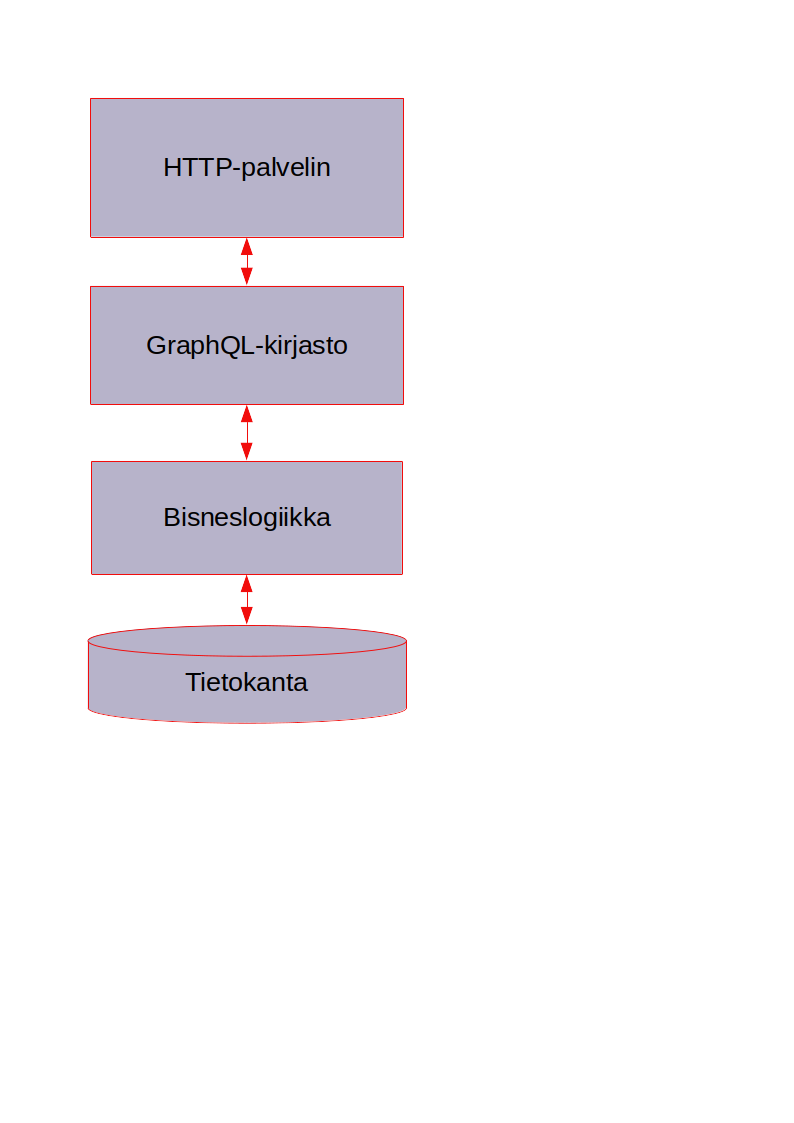
\includegraphics{illustration/GraphQL-arkkitehtuuri.png}
\caption{\label{graphqlarkkitehtuuri} Esimerkkiarkkitehtuuri
GraphQL-sovellukselle}
\end{figure}

Kuvassa \ref{graphqlarkkitehtuuri} esitän yksinkertaisen
GraphQL-sovelluksen arkkitehtuurin. Arkkitehtuuri on kerroksittainen, ja
rajapinnalle esitettävä pyyntö liikkuu siinä ylhäältä alaspäin. Koska
GraphQL on teknologianeutraali, tämä on vain yksi, toki suhteellisen
tyypillinen esimerkki mahdollisesta GraphQL-sovelluksesta.

Ensiksi pyyntö saapuu HTTP-palvelimeen. Tämä palvelin on käytännössä
ohjelmointikielestä riippuen kirjasto, joka vastaanottaa HTTP-pyyntöjä
ja osaa käsitellä niitä. Tyypillisesti GraphQL-rajapinnassa on vain yksi
\texttt{graphql}-niminen resurssi, jolle pyynnöt esitetään. Pyynnöt ovat
aina POST-tyyppisiä.

HTTP-kerros ottaa pyynnön vastaan, ja lukee sen body-osassa olevan
merkkijonomuotoisen GraphQL-kyselyn. Tämä kysely on tehty
GraphQL-kyselykielellä. Rajapinta antaa kyselyn GraphQL-kirjastolle.

Kirjasto ottaa kyselyn vastaan, ja tarkistaa sen oikeellisuuden
GraphQL-skeemaa vasten. Mikäli kysely on muodoltaan oikeanlainen,
kirjasto ohjaa sen eteenpäin resolvereiksi kutsutuille funktioille.
Resolver-funktiot eivät ole osa kirjastoa, vaan sovelluksen kehittäjä
kirjoittaa ne. Käytännössä resolver-funktio on nk. \gls{puhdasfunktio},
jonka tehtävänä on tuottaa vastaus yksittäiseen GraphQL-kyselyn
kenttään.

Laskutusta käsittelevässä esimerkissä rajapinnan invoices-kenttää voisi
vastata \texttt{invoices\_resolver} -niminen funktio.

Resolver-funktioiden kerros on alin kerros, josta GraphQL-palvelu
tietää. Sen alla oleva ohjelmistologiikka on riippumaton rajapinnan
olemassaolosta. Tyypillisesti siellä voi sijaita sovelluksen
liiketoimintalogiikka ja infrastruktuuri, kuten esimerkiksi tiedon
tallennusteknologia.

\hypertarget{query-ja-mutation--juurityypit}{%
\subsection{Query ja Mutation
-juurityypit}\label{query-ja-mutation--juurityypit}}

GraphQL-palveluissa on muutama oletuksena määritelty tyyppi, joita
kutsutaan juurityypeiksi. Tässä käsittelen niistä kahta keskeisintä,
Query- ja Mutation-tyyppiä.

Rajapintaan voi tehdä kyselyjä Query-tyyppisen juuriolion kautta. Tämän
olion kentät määrittävät, mitä dataa rajapinnalta voidaan kysellä.
Kentät ovat ikäänkuin sisäänmenoaukkoja, joiden kautta oliorakenteita
voi pyytää.

Kun aiemman koodiesimerkin \ref{listing1} mukaisesti määritellystä
GraphQL-rajapinnasta halutaan hakea tietoja, tehdään Query-tyypin
consolidatedInvoices -kenttään kysely, joka kuvaa halutun oliopuun
rakenteen tyyppien avulla. Tätä kuvaa koodiesimerkki \ref{listing2}.

\begin{code}
  \begin{minted}{graphql}

{
  consolidatedInvoices {
    number
    invoices {
      number
      sum
    }
  }
}
\end{minted}
\captionof{listing}{Kysely, joka pyytää consolidatedInvoices-olioita}
  \label{listing2}
\end{code}

Kyselyssä määritellään kentät, jotka palautuvassa datassa halutaan
nähdä. Näin myös palautuvan oliopuun syvyyttä voidaan kontrolloida.
Oheisessa esimerkissä haetaan paitsi lista koontilaskuista, myös
jokaisen koontilaskun alle invoices-kenttään lista siihen kuuluvista
laskuista. Niistä pyydetään jokaisesta laskunumero ja laskun summa. Näin
edetään verkkoa pitkin tarvittavan datan luo.

Mutation-juurityyppiä puolestaan käytetään datan muunnoksiin.
Mutation-tyypin sisältämiin kenttiin lähetetään kysely, jossa mukana
olevat parametrit kertovat, miten dataa muokataan. Parametrit ovat yhtä
lailla tyypitettyjä kuin rajapinnan kentät, ja GraphLQ-kirjasto
tarkistaa niiden tyypin oikeellisuuden. Mutation-komennot voivat myös
palauttaa oliorakenteita.

Oheisessa koodiesimerkissä \ref{listing3} määritellään invoice-niminen
operaatio uuden laskun luomiseen. Operaatiolle on merkitty paluuarvo,
joka on Invoice-tyyppinen olio. Käytännössä operaatio siis palauttaa
juuri luodun laskun.

\begin{code}
  \begin{minted}{graphql}
Mutation {
  invoice(customerId: Int, appointmentDate: String): Invoice
}
\end{minted}
\captionof{listing}{Esimerkki GraphQL-mutaatiosta}
  \label{listing3}
\end{code}

Kun tällaista mutaatiota käytetään, kutsuun liitetään myös kyselyosa,
jossa listataan ne kentät, jotka palautuvasta oliosta halutaan.
Koodiesimerkissä \ref{listing4} pyydetään laskunumero ja laskun summa.

\begin{code}
  \begin{minted}{graphql}

{
invoice(customerId: 1, appoitnmentDate: "2021-09-21") {
    number
    sum
  }
}
\end{minted}
\captionof{listing}{Esimerkki parametreja käyttävästä GraphQL-kyselystä}
  \label{listing4}
\end{code}

\hypertarget{graphql-ja}{%
\section{\texorpdfstring{GraphQL ja
\glsentryname{ddd}}{GraphQL ja }}\label{graphql-ja}}

Eric Evansin kirjassa \glsentryname{domainmodel} rakennetaan
olio-ohjelmoinnin tekniikoita käyttäen. Vaikka se ei olekaan ainoa tapa
rakentaa \glsentryname{domainmodel}, on se kuitenkin tyylinä hyvin
suosittu.

Kuten edellä olen esittänyt, GraphQL puolestaan on olioverkkoon
perustuva rajapinta, jossa rajapinnan tarjoama tieto on jäsennetty
olioiksi ja niiden välisiksi suhteiksi.

Voidaan siis esittää kysymys, kuinka hyvin GraphQL-rajapinta soveltuu
\glsdisp{ddd}{sovellusaluevetoisen suunnittelun} tarpeisiin? On helppo
kuvitella, että olioverkolla on mahdollista heijastaa
\glsentryname{domainmodel}, ja jopa mallintaa se lähes yksi yhteen.
Toisaalta GraphQL-rajapinta palauttaa dataa, kun taas olio-ohjelmoinnin
keinon luotu olioverkko voi esittää dynaamisen ja muuttuvan mallin. Onko
GraphQL toimiva väline ohjelmiston tietomallin parantamiseen? Tätä
kysymystä lähden työni käytännön osassa selvittämään.
